The wide availability and reduced cost of molecular marker technology
has created opportunities to perform marker assisted selection of genotypes
in plant and animal breeding. Quantitative Trait Locus (QTL) mapping techniques
have proved useful for detecting the effects of small numbers of markers producing 
phenotypes with large effects \citep{miles2008}. Once the QTL 
markers have been identified, they can be leveraged for making selections
on a population. However, when making selections on traits affected by many 
alleles with varying effect sizes distributed widely across a genome, 
QTL mapping is less effective. 

Unlike QTL mapping, genomic selection methods attempt to predict phenotypes 
utilizing all available SNP marker data collected from a population,
allowing one of many possible statistical models to learn the marker-trait 
associations in a data driven way \citep{meuwissen2001}. This techique has
proven effective but relies on an appropriate choice of the statistical 
model that will most accurately predict phenotype from a panel of high-density 
marker data. It is likely that the best statistical model for 
genomic selection is dependent on the genetic archetecture of the 
predicted trait \citep{crossa2010, gonzalez-camacho2012, 
resende2012, cleveland2012, thavamanikumar2015}.  Mathematically, models incorporating 
interactions between marker features have the capacity to achieve higher accuracy 
by caputuring non-additive effects. Experimental results support this 
hypothesis \citep{gonzalez-camacho2012}. Alternative prediction methods continue 
to be an active area of research in plant and animal breeding \citep{koning2012}.

Concurrent with the advent of genomic selection as a practice the popularity of the 
interdisciplinary field known as data science has increased. Practitioners of data 
science apply machine learning and statistics to make predictions, usually
by applying ideas or techniques from a wide variety of domains 
including mathematics, physics, and computer science. Often, a data scientist's focus is to
create a predictive model than may not be associated with an underlying generative model. 
This can be viewed as the distinction between data science and classical statistics 
\citep{donoho2015, breiman2001}. The rapid increase in popularity of data science
is associated with an increase in definition of best practices for predictive modeling
across many disciplines as well as software packages to automate the 
process of building predictive models from any data source.

Neural networks are a type of model frequently employed by data scientists
for predictive modeling. Neural networks consist of layers of interconnected neurons
which map inputs to one or more outputs. Each neuron in a network can be expressed as a 
transformation of a weighted sum of $n$ inputs 

\begin{equation}
output_{lk} = \sum_{i=1}^{n} f_l(w_{lki} * x_{i} + b_{lk})
\label{eq:neuron}
\end{equation}

where $output_{lk}$ is the output from neuron $k$ in network layer $l$ having activation
function $f_l$, weights $w_{lki}$ and bias $b_{lk}$.

A neural network is a collection of neurons that map a 
length $n$ input vector $x = (x_1, ..., x_n)$ through a series of $j$ 
"hidden" layers $(l_1, ..., l_j)$. Each hidden layer consists of a variable 
number of neurons, each of which apply an associated coefficient, bias, and 
mathematical transformation to their input and forward the 
result on to every neuron in the subsequent layer forming a network (Figure \ref{fig:deepnet}).

\ifdefined\showtablesandfigures
% A deep neural network with 3 hidden layers of varying sizes.

\def\layersep{1.5cm}

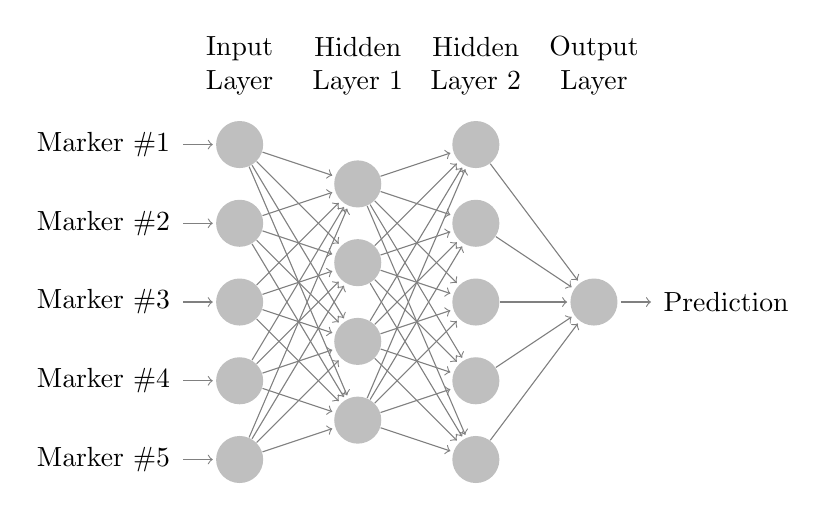
\begin{tikzpicture}[shorten >=1pt, ->, draw=black!50, node distance=\layersep]
    \tikzstyle{every pin edge}=[<-, shorten <=1pt]

    \tikzstyle{neuron}=[circle, fill=black!25,minimum size=17pt, inner sep=0pt]
    \tikzstyle{input neuron}=[neuron];
    \tikzstyle{output neuron}=[neuron];
    \tikzstyle{hidden neuron}=[neuron];

    \tikzstyle{annot}=[text width=4em, text centered]

    \foreach \name / \y in {1,...,5}
        \node[input neuron, pin=left:Marker \#\y] (I-\name) at (0,-\y) {};

    \foreach \name / \y in {1,...,4}
        \path[yshift=-0.5cm]
            node[hidden neuron] (H1-\name) at (\layersep * 1,-\y cm) {};

    \foreach \name / \y in {1,...,5}
        \path[yshift=0.0cm]
            node[hidden neuron] (H2-\name) at (\layersep * 2,-\y cm) {};

    \node[output neuron, pin={[pin edge={->}]right:Prediction}, right of=H2-3] (0) {};

    \foreach \source in {1,...,5}
        \foreach \dest in {1,...,4}
            \path (I-\source) edge (H1-\dest);

    \foreach \source in {1,...,4}
        \foreach \dest in {1,...,5}
            \path (H1-\source) edge (H2-\dest);

    \foreach \source in {1,...,5}
        \path (H2-\source) edge (0);

    \node[annot, above of=I-1, node distance=1cm] (il) {Input Layer};
    \node[annot, right of=il] (hl1) {Hidden Layer 1};
    \node[annot, right of=hl1] (hl2) {Hidden Layer 2};
    \node[annot, right of=hl2] {Output Layer};
\end{tikzpicture}

 % Label = fig:deepnet
\fi

Once the network is defined, it must be exposed to input and desired output
values, and adjusted to minimize error in output in a process known as training.
Error in the output of the network is propagated back through the hidden 
layers, and the weights and biases are updated in the direction that would 
decrease output error on many sets or subsets of the input data. 
This turns the network training process into general 
function minimization problem, where the parameters to the function are the 
weights and biases of the network neurons and the function to be 
minimized is the squared differences between the network outputs and 
the desired outputs. The process of propagating output error back 
through a neural network is known as backpropagation, and has been used 
and improved extensively since its description in the 1980s \citep{rumelhart1986}. 

%Good post, good links to the 'deep' part of deep nets.
%http://stats.stackexchange.com/questions/182734/what-is-the-difference-between-a-neural-network-and-a-deep-neural-network

Networks with many hidden layers are notoriously difficult to train due to
the vanishing gradient problem \citep{hochreiter1998}. Recently, a series 
of breakthroughs in neural network training have allowed efficient 
training of deeper networks than were previously possible \citep{sutskever2013}.
A history of the deep learning literature is available in \cite{lecun2015}.
The increased training efficiency and potential to capture relationships 
between input features drove a need to differentiate these deeper networks
from prior work, resulting in the emergence of the phrase "deep learning" 
to describe the construction and training of deep neural networks.

Attempts to apply neural networks to genomic selection has resulted in overfitting of the 
network to training data as well as concerns over the 
computation complexity required to fit the model to datasets with many
markers across many genotypes \citep{heslot2012, gonzalez-recio2014}. 
These results are not surprising. Multi-layer feedforward neural networks 
are capable of approximating functions of arbitrary complexity to arbitrary 
accuracy if provided enough neurons in even a single hidden 
layer. This property of neural networks is known as the 
universal approximation theorem, and can result in 
overfitting if the weights of the network are not regularized in some way \citep{hornik1989}.

Given the promising results from regularized and bayesian methods for 
genomic selection such as ridge or lasso regression and the bayesian family of regressors,
it is prudent to evaluate some of the many of neural network training algorithms which
incorporate regularization of weights during training. Today, networks based on these 
and other regularization techniques continue to achieve award-winning performance 
across many domains \citep{schmidhuber2015}. Similarly, while neural networks are 
computationally demanding to train, the training algorithms 
themselves are often easily expressed with vector and matrix algebra and thus amenable to
Graphics Processing Unit (GPU) accelerated computing. Some report up to sixty-fold speedups 
in training time \citep{sierra2010, schmidhuber2015}. 

In this paper, we present the results of applying two types of regularization
to deep neural networks. The first is a weight decay regularization
which penalizes the weights $W$ with very large values 
similar to ridge regression \citep{krogh1992}. The second is known as dropout 
regularization, where subsets of neurons and their connections are removed 
at random during training, encouraging subsets of the network to learn 
to recognize input features independently. This allows neurons to adapt 
and build independently operating units and prevents the 
neurons from co-adapting, reducing overfitting \citep{srivastava2014}.  

% For the introduction, authors should be mindful of the broad readership of the journal. i
% The introduction should set the stage for the importance of the work to a generalist 
% reader and draw the reader in to the specific study. The scope and impact of the 
% work should be clearly stated.

